\documentclass[12pt]{article}
\usepackage{polski}
\usepackage[utf8]{inputenc}
\usepackage{fullpage}
\usepackage{tabto}
\usepackage{graphicx} 
\usepackage{float}
\usepackage{caption}
\usepackage{indentfirst}



\linespread{1.3}
\begin{document}

%---------------------------------------------------------
%					Strona Tytułowa
%---------------------------------------------------------
\begin{titlepage}
%-----------------------Tytuł-----------------------------

 \newcommand{\LINE}{\rule{\linewidth}{0.1mm}}
\begin{center}
 \LARGE  POLITECHNIKA WROC\L{}AWSKA \\[0mm] %
  WYDZIAŁ ELEKTRONIKI            %
  \vspace{-6mm}%
  
  \LINE \\[0.1cm]
\end{center}

\textsc{Kierunek:}  \hspace{15mm} Informatyka (INF) \\[0.5cm]

\begin{center}
\large \textbf{ZASTOSOWANIA INFORMATYKI} \\
\textbf{W GOSPODARCE} \\ [1cm]
\end{center}

\normalsize

%----------------------Nazwiska---------------------------
\begin{center}
\hspace{55mm}Cyfrowa historia pojazdu\\[0.5cm]
\hspace{55mm}Digital vehicle history \\[0.5cm]
\hspace{55mm}\textsc{Autorzy:}  \\[0.1cm]
\hspace{55mm}Grzegorz Milaszkiewicz \\
\hspace{55mm}Mateusz Ożóg \\
\hspace{55mm}Igor Kurek\\
\hspace{55mm}Piotr Wodzyński\\
\hspace{55mm}Maciej Kucia \\[2.0cm]

\hspace{5mm}\textsc{Prowadzący:} \\
\hspace{15mm}dr inż. Marek Woda \\[1.2cm]

\hspace{6mm}\textsc{Ocena pracy:} \\[1.72cm]

\end{center}


%----------------------Stopka-----------------------------
%\vfill
\LINE
\center Wrocław 2019
\end{titlepage}
%---------------------------------------------------------
%					Spis treści
%---------------------------------------------------------
\renewcommand{\contentsname}{Spis treści}
\tableofcontents
\newpage

%---------------------------------------------------------
%					Część pierwsza
%---------------------------------------------------------
\section{Temat projektu}

Tematem projektu jest system umożliwiający dokumentowanie historii pojazdów. Obecnie rynek samochodów używanych jest kojarzony z tak zwanym pojęciem "kręcenia liczników", czyli zmniejszania faktycznego przebiegu pojazdu w celu podwyższenia jego wartości. Usługa korekty licznika jest stosunkowo tania i trudno wykrywalna. Najbardziej na tego typu zabiegach cierpią uczciwi posiadacze samochodów, którzy mają trudność w sprzedaży pojazdów z~oryginalnym przebiegiem. System do dokumentowania historii pojazdów umożliwiłby uczciwym sprzedawcom podniesienie wartości swoich pojazdów. \\

Pomysł dokumentowania historii pojazdu nie jest pomysłem innowacyjnym. Na rynku jest wiele aplikacji umożliwiających zapisywanie historii pojazdów, jednakże żadna z nich nie weryfikuje wprowadzanych danych. Wszystkie aplikacje oferowane przez konkurencję są nastawione tylko na informowanie właściciela pojazdu o jego wydatkach na samochód. Jest to ich główna i jedyna funkcjonalność, która mogłaby zostać rozszerzona tak, aby czas poświęcony na dokumentowanie historii pojazdu zwrócił się kiedyś właścicielowi samochodu.\\

System\textit{ Cyfrowa historia pojazdu} będzie posiadał podobne funkcjonalności co inne aplikacje dostępne na rynku, lecz dodatkowo wymaga wprowadzenia przebiegu pojazdu przy każdym wpisie do bazy danych. Kolejną funkcjonalnością potwierdzającą dodanie wpisu będzie możliwość dodania zdjęcia (na przykład zdjęcia licznika pojazdu). Zwiększy to wiarygodność wpisów, a co za tym idzie zostanie zwiększona autentyczność całej historii pojazdu. Uczciwy posiadacz samochodu zyska na tym więcej niż nieuczciwy handlarz zyskuje na sprzedaży pojazdów z zaniżonym przebiegiem, gdyż ludzie chętniej będą kupowali pojazdy ze zweryfikowaną przeszłością. Aplikacja przy odpowiedniej promocji może przyczynić się do wyeliminowania nieuczciwych handlarzy. Osoba, która będzie chciała korzystać z systemu i jednocześnie fałszować przebieg będzie musiała dokonywać korekty licznika przed każdym wpisem co będzie dla niej nieopłacalne. 




%---------------------------------------------------------
%					Część druga
%---------------------------------------------------------
\newpage
\section{Zakres projektu}
\subsection{Cele}
Celem projektu jest stworzenie systemu umożliwiającego dokumentowanie histroii pojazdów. Głównym zadaniem jest napisanie aplikacji mobilnej i webowej, która będzie przyjazna dla użytkownika. Aplikacja webowa będzie przeznaczona dla właścicieli pojazdów oraz dla serwisów samochodowych, zaś aplikacja mobilna będzie przeznaczona tylko dla właścicieli pojazdów.
\subsection{Ryzyka}
Projektując taki system należy liczyć się z nieuniknionym ryzykiem. Głównym niebezpieczeństwem projektowanego systemu jest niskie lub całkowity brak zainteresowania ze strony użytkowników. Jest to dość realne zagrożenie z uwagi na mnogość tego typu aplikacji, które pomimo braku weryfikacji wprowadzanych informacji są o wiele bardziej wypromowane. Aby zminimalizować możliwość wystąpienia tego ryzyka należy stworzyć jak najbardziej przyjazną dla użytkowników aplikację, która będzie łatwa w obsłudze. Najlepszą promocją aplikacji będzie rekomendacja ze strony użytkowników. System \textit{ Cyfrowa historia pojazdu} ma szanse konkurować z innymi rozwiązaniami dostępnymi na rynku dzięki jego prostej obsłudze.

Kolejnym ryzykiem jest opóźnienie w wykonywaniu pracy. Jest to istotne niebezpieczeństwo, które może wyniknąć ze zbyt dużej ilości funkcjonalności oraz z niedostatecznej wiedzy programistycznej w wybranych technologiach. W celu redukcji możliwości wystąpienia tego zagrożenia należy często weryfikować postęp prac z zaplanowanym harmonogramem, a gdy tylko wystąpią jakieś opóźnienia należy od razu zwiększyć nakład pracy.

Następnym ryzykiem jest zmiana założonych funkcjonalności podstawowych systemu. Każda nieprzewidziana zmiana niesie za sobą spore konsekwencje. Nawet niewielka modyfikacja założeń projektowych może spowodować opóźnienia w planowanym ukończeniu projektu. Żeby zminimalizować możliwość wystąpienie tego ryzyka należy dobrze przemyśleć i~opisać podstawowe funkcjonalności systemu. Jednakże, gdy konieczna będzie zmiana założeń w celu zachowania terminów zgodnych z harmonogramem należy zrezygnować z jakiejś funkcjonalności lub ją uprościć.

\subsection{Funkcjonalności podstawowe i rozszerzone}

W tabelach 1-10 zostały przedstawione podstawowe funkcjonalności systemu, a w tabelach 11-15 funkcjonalności rozszerzone.

%----------------------REJESTRACJA------------------------------------
\begin{table}[H]
\begin{center}
\captionof{table}{Karta wymagań dla funkcjonalności \textit{Rejestracja konta}} 
	\begin{tabular}{|p{0.18\linewidth}|p{0.72\linewidth}|}%{|l|l|}
	\hline
	Id wymagania 	& 1 				\\ \hline
	Nazwa			& Rejestracja konta \\ \hline
	Opis & Aplikacja powinna zarejestrować użytkownika po wypełnieniu
formularza rejestracyjnego\\ \hline
	Przesłanka & Możliwość dodawania nowych użytkowników  \\ \hline
	Ograniczenia i~warunki & Rejestracja nowych użytkowników może odbyć się tylko po potwierdzeniu adresu e-mail  \\ \hline
	Dane wejściowe & Typ konta: 1. Właściciel pojazdu, 2. Serwis \\
	&  1. Imię, nazwisko, email, hasło \\
	& 2. Nazwa serwisu, adres (ulica, kod pocztowy, miasto), adres email, hasło  \\ \hline
	Wynik & Dodanie nowego użytkownika do systemu \\ \hline
	Źródło danych wejściowych & Użytkownik (Właściciel pojazdu, Serwis samochodowy, Osoba zewnętrzna) \\ \hline
	Przeznaczenie & Każdy nowy użytkownik \\ \hline
	Priorytet & Funkcjonalność podstawowa \\ \hline
	\end{tabular}

\end{center}
\end{table}

%----------------------LOGOWANIE------------------------------------
\begin{table}[H]
\begin{center}
\captionof{table}{Karta wymagań dla funkcjonalności \textit{Logowanie}} 
\end{center}
	\begin{tabular}{|p{0.18\linewidth}|p{0.72\linewidth}|}%{|l|l|}
	\hline
	Id wymagania 	& 2 				\\ \hline
	Nazwa			& Logowanie \\ \hline
	Opis & Aplikacja powinna zalogować użytkownika do systemu po
podaniu poprawnych danych logowania
\\ \hline
	Przesłanka & Jednoznaczne zidentyfikowanie użytkownika  \\ \hline
	Ograniczenia i~warunki & Weryfikacja użytkownika powinna zapewnić poufność i bezpieczeństwo procesu  \\ \hline
	Dane wejściowe & Dane niezbędne do identyfikacji i weryfikacji użytkownika
w systemie - login (adres e-mail) i hasło użytkownika
  \\ \hline
	Wynik & Zalogowanie do systemu \\ \hline
	Źródło danych wejściowych & Użytkownik (Właściciel pojazdu, Serwis samochodowy, Osoba zewnętrzna) \\ \hline
	Przeznaczenie & Każdy zarejestrowany użytkownik \\ \hline
	Priorytet & Funkcjonalność podstawowa \\ \hline
	\end{tabular}

\end{table}

%----------------------REJESTRACJA POJAZDU------------------------------------
\begin{table}[H]
\begin{center}
\captionof{table}{Karta wymagań dla funkcjonalności \textit{Rejestracja pojazdu}} 
	\begin{tabular}{|p{0.18\linewidth}|p{0.72\linewidth}|}%{|l|l|}
	\hline
	Id wymagania 	& 3 				\\ \hline
	Nazwa			& Przeglądanie pojazdów \\ \hline
	Opis & Aplikacja powinna umożliwić przeglądanie pojazdów w systemie. Właściciel pojazdów ma mieć możliwość zobaczenia jakie pojazdy są zarejestrowane do jego konta
\\ \hline
	Przesłanka & Możliwość przejrzenia swoich pojazdów  \\ \hline
	Ograniczenia i~warunki & Właściciel pojazdów może zobaczyć tylko swoje samochody  \\ \hline
	Dane wejściowe & Brak  \\ \hline
	Wynik & Lista wszystkich pojazdów właściciela \\ \hline
	Źródło danych wejściowych & Użytkownik (Właściciel pojazdu) \\ \hline
	Przeznaczenie & Właściciel pojazdu \\ \hline
	Priorytet & Funkcjonalność podstawowa \\ \hline
	\end{tabular}

\end{center}
\end{table}


%----------------------PRZEGLĄDANIE POJAZDÓW------------------------------------
\begin{table}[H]
\begin{center}
\captionof{table}{Karta wymagań dla funkcjonalności \textit{Przeglądanie pojazdów}} 
	\begin{tabular}{|p{0.18\linewidth}|p{0.72\linewidth}|}%{|l|l|}
	\hline
	Id wymagania 	& 4 				\\ \hline
	Nazwa			& Rejestracja pojazdu \\ \hline
	Opis & Aplikacja powinna umożliwić zarejestrowanie pojazdu w systemie. Zarejestrowanie pojazdu odbywać się będzie poprzez podanie kilku informacji na temat pojazdu
\\ \hline
	Przesłanka & Możliwość dodawania pojazdów do bazy danych  \\ \hline
	Ograniczenia i~warunki & Pojazd można dodać tylko po poprawnym wprowadzeniu danych.  \\ \hline
	Dane wejściowe &
Dane niezbędne do identyfikacji pojazdu - numer rejestracyjny, numer nadwozia, data pierwszej rejestracji w kraju
(opcjonalne: zdjęcie pojazdu)  \\ \hline
	Wynik & Dodanie pojazdu do systemu \\ \hline
	Źródło danych wejściowych & Użytkownik (Właściciel pojazdu) \\ \hline
	Przeznaczenie & Właściciel pojazdu \\ \hline
	Priorytet & Funkcjonalność podstawowa \\ \hline
	\end{tabular}

\end{center}
\end{table}

%----------------------DODAWANIE NAPRAW------------------------------------
\begin{table}[H]
\begin{center}
\captionof{table}{Karta wymagań dla funkcjonalności \textit{Dodawanie napraw pojazdu}} 
	\begin{tabular}{|p{0.18\linewidth}|p{0.72\linewidth}|}%{|l|l|}
	\hline
	Id wymagania 	& 5				\\ \hline
	Nazwa			& Dodawanie napraw pojazdu \\ \hline
	Opis & Aplikacja powinna umożliwić dodanie informacji o naprawie pojazdu
\\ \hline
	Przesłanka & 
Możliwość dodawania informacji o historii pojazdu
  \\ \hline
	Ograniczenia i~warunki & 
Każda naprawa musi zawierać informację o przebiegu pojazdu w chwili dokonania naprawy oraz opis co zostało naprawione
 \\ \hline
	Dane wejściowe &

Przebieg pojazdu, opis naprawy
(opcjonalne: zdjęcia, kwota naprawy)
 \\ \hline
	Wynik & Dodanie informacji o naprawie pojazdu wraz z informacją kto dodał naprawę\\ \hline
	Źródło danych wejściowych & Użytkownik (Właściciel pojazdu, Serwis samochodowy)\\ \hline
	Przeznaczenie & Właściciel pojazdu, Serwis samochodowy\\ \hline
	Priorytet & Funkcjonalność podstawowa \\ \hline
	\end{tabular}

\end{center}
\end{table}

%----------------------DODAWANIE EKSPLOATACJI------------------------------
\begin{table}[H]
\begin{center}
\captionof{table}{Karta wymagań dla funkcjonalności \textit{Dodawanie eksploatacji pojazdu}} 
	\begin{tabular}{|p{0.18\linewidth}|p{0.72\linewidth}|}%{|l|l|}
	\hline
	Id wymagania 	& 6 				\\ \hline
	Nazwa			& Dodawanie eksploatacji pojazdu \\ \hline
	Opis &	 Aplikacja powinna umożliwić dodanie informacji o wymianach eksploatacyjnych pojazdu (np. wymiana oleju)\\ \hline
	Przesłanka & Możliwość dodawania informacji o historii pojazdu  \\ \hline
	Ograniczenia i~warunki & Każda wymiana eksploatacyjna musi zawierać informację o przebiegu pojazdu w chwili dokonania wymiany oraz opis co zostało wymienione \\ \hline
	Dane wejściowe &Przebieg pojazdu, opis wymiany eksploatacyjnej
(opcjonalne: zdjęcia, kwota wymiany eksploatacyjnej) \\ \hline
	Wynik & Dodanie informacji o wymianie eksploatacyjnej pojazdu wraz z informacją kto dodał wymiany\\ \hline
	Źródło danych wejściowych &Użytkownik (Właściciel pojazdu, Serwis samochodowy)\\ \hline	Przeznaczenie & Właściciel pojazdu, Serwis samochodowy\\ \hline
	Priorytet & Funkcjonalność podstawowa \\ \hline
	\end{tabular}
\end{center}
\end{table}

%----------------------DODAWANIE ULEPSZEŃ------------------------------------
\begin{table}[H]
\begin{center}
\captionof{table}{Karta wymagań dla funkcjonalności \textit{Dodawanie ulepszeń}} 
	\begin{tabular}{|p{0.18\linewidth}|p{0.72\linewidth}|}%{|l|l|}
	\hline
	Id wymagania 	& 7 				\\ \hline
	Nazwa			& Dodawanie ulepszeń
 \\ \hline
	Opis &	Aplikacja powinna umożliwić dodanie informacji o ulepszeniach pojazdu (np. przyciemnianie szyb)\\ \hline
	Przesłanka & Możliwość dodawania informacji o historii pojazdu  \\ \hline
	Ograniczenia i~warunki & Każde ulepszenie musi zawierać informację o przebiegu pojazdu w chwili dokonania ulepszenia oraz opis co zostało ulepszone \\ \hline
	Dane wejściowe &Przebieg pojazdu, opis ulepszeń
(opcjonalne: zdjęcia, kwota dokonania ulepszenia) \\ \hline
	Wynik & Dodanie informacji o ulepszeniach pojazdu wraz z informacją kto dodał ulepszenia\\ \hline
	Źródło danych wejściowych &Użytkownik (Właściciel pojazdu, Serwis samochodowy)\\ \hline
	Przeznaczenie &Właściciel pojazdu, Serwis samochodowy\\ \hline
	Priorytet & Funkcjonalność podstawowa \\ \hline
	\end{tabular}
\end{center}
\end{table}

%----------------------DODAWANIE USZKODZEŃ------------------------------------
\begin{table}[H]
\begin{center}
\captionof{table}{Karta wymagań dla funkcjonalności \textit{Dodawanie uszkodzeń}} 
	\begin{tabular}{|p{0.18\linewidth}|p{0.72\linewidth}|}%{|l|l|}
	\hline
	Id wymagania 	& 8 				\\ \hline
	Nazwa			& Dodawanie uszkodzeń \\ \hline
	Opis &Aplikacja powinna umożliwić dodanie informacji o uszkodzeniach pojazdu (np. pęknięcie szyby)\\ \hline
	Przesłanka & Możliwość dodawania informacji o historii pojazdu  \\ \hline
	Ograniczenia i~warunki & Każde uszkodzenie musi zawierać informację o przebiegu pojazdu w chwili wystąpienia uszkodzenia oraz opis co uległo uszkodzeniu \\ \hline
	Dane wejściowe &Przebieg pojazdu, opis uszkodzeń
(opcjonalne: zdjęcia)\\ \hline
	Wynik & Dodanie informacji o uszkodzeniach pojazdu\\ \hline
	Źródło danych wejściowych &Użytkownik (Właściciel pojazdu)\\ \hline
Przeznaczenie & Właściciel pojazdu\\ \hline
Priorytet & Funkcjonalność podstawowa \\ \hline
	\end{tabular}
\end{center}
\end{table}


%----------------------SPRZEDAWANIE------------------------------------
\begin{table}[H]
\begin{center}
\captionof{table}{Karta wymagań dla funkcjonalności \textit{Sprzedaż samochodu}} 
	\begin{tabular}{|p{0.18\linewidth}|p{0.72\linewidth}|}%{|l|l|}
	\hline
	Id wymagania 	& 9 				\\ \hline
	Nazwa			& Sprzedaż samochodu \\ \hline
	Opis &Aplikacja powinna umożliwić sprzedaż pojazdu, czyli przypisanie pojazdu do innego konta
\\ \hline
	Przesłanka & Możliwość zmiany właściciela pojazdu  \\ \hline
	Ograniczenia i~warunki & Przypisać pojazd można tylko do zweryfikowanego konta po wprowadzeniu adresu email nowego właściciela. Nowy właściciel musi potwierdzić dokonanie zmiany właściciela. \\ \hline
	Dane wejściowe &Adres email nowego właściciela \\ \hline
	Wynik & Zmiana właściciela pojazdu\\ \hline
	Źródło danych wejściowych &Użytkownik (Właściciel pojazdu)\\ \hline
	Przeznaczenie & Właściciel pojazdu\\ \hline
	Priorytet & Funkcjonalność podstawowa \\ \hline
	\end{tabular}
\end{center}
\end{table}

%----------------------UDOSTĘPNIANIE HISTORII--------------------------------
\begin{table}[H]
\begin{center}
\captionof{table}{Karta wymagań dla funkcjonalności \textit{Udostępnienie historii samochodu}} 
	\begin{tabular}{|p{0.18\linewidth}|p{0.72\linewidth}|}%{|l|l|}
	\hline
	Id wymagania 	& 10 				\\ \hline
	Nazwa			& Udostępnienie historii samochodu \\ \hline
	Opis &	Aplikacja powinna umożliwić udostępnienie historii pojazdu. Historia pojazdu powinna zawierać wszystkie informacje wprowadzone przez właściciela pojazdu oraz serwisy samochodowe. Każdy wpis powinien zawierać opis, datę oraz przebieg w momencie dodania wpisu. Aplikacja powinna generować plik PDF zawierający historię pojazdu \\ \hline
	Przesłanka & Możliwość udostępnienia historii pojazdu potencjalnemu nabywcy   \\ \hline
	Ograniczenia i~warunki & Właściciel może udostępnić historię tylko tych pojazdów które posiada \\ \hline
	Dane wejściowe &Wybór pojazdu którego historia ma zostać udostępniona \\ \hline
	Wynik & Plik PDF umożliwiający zobaczenie wszystkich wpisów dla danego pojazdu\\ \hline
	Źródło danych wejściowych &Użytkownik (Właściciel pojazdu)\\ \hline
	Przeznaczenie & Właściciel pojazdu\\ \hline
	Priorytet & Funkcjonalność podstawowa \\ \hline
	\end{tabular}
\end{center}
\end{table}
%-------------------FUNKCJONALNOŚCI ROZSZERZONE---------------------------
%----------------------ZMIANA NR REJESTRACYJNEGO------------------------------------
\begin{table}[H]
\begin{center}
\captionof{table}{Karta wymagań dla funkcjonalności \textit{Zmiana numeru rejestracyjnego}} 
	\begin{tabular}{|p{0.18\linewidth}|p{0.72\linewidth}|}%{|l|l|}
	\hline
	Id wymagania 	& 11 				\\ \hline
	Nazwa			& Zmiana numeru rejestracyjnego \\ \hline
	Opis &Aplikacja powinna umożliwić zmianę numeru rejestracyjnego pojazdu
\\ \hline
	Przesłanka & Możliwość aktualizacji numeru rejestracyjnego pojazdu  \\ \hline
	Ograniczenia i~warunki & Zmienić numer rejestracyjny może tylko właściciel pojazdu \\ \hline
	Dane wejściowe & Nowy numer rejestracyjny \\ \hline
	Wynik & Zmiana numeru rejestracyjnego\\ \hline
	Źródło danych wejściowych &Użytkownik (Właściciel pojazdu)\\ \hline
	Przeznaczenie & Właściciel pojazdu\\ \hline
	Priorytet & Funkcjonalność rozszerzona \\ \hline
	\end{tabular}
\end{center}
\end{table}
%----------------------TANKOWANIE------------------------------------
\begin{table}[H]
\begin{center}
\captionof{table}{Karta wymagań dla funkcjonalności \textit{Historia tankowania}} 
	\begin{tabular}{|p{0.18\linewidth}|p{0.72\linewidth}|}%{|l|l|}
	\hline
	Id wymagania 	& 12 				\\ \hline
	Nazwa			& Historia tankowania \\ \hline
	Opis &Aplikacja powinna umożliwić dodanie informacji o tankowaniach pojazdu
\\ \hline
	Przesłanka & Możliwość dodania informacji o tankowaniu pojazdu  \\ \hline
	Ograniczenia i~warunki & Informację o tankowaniu może dodać tylko właściciel pojazdu \\ \hline
	Dane wejściowe & Przebieg, rodzaj zatankowanego paliwa, objętość zatankowanego paliwa, kwota \\ \hline
	Wynik &Dodanie informacji o tankowaniu pojazdu\\ \hline
	Źródło danych wejściowych &Użytkownik (Właściciel pojazdu)\\ \hline
	Przeznaczenie & Właściciel pojazdu\\ \hline
	Priorytet & Funkcjonalność rozszerzona \\ \hline
	\end{tabular}
\end{center}
\end{table}
%----------------------OŚ CZASU------------------------------------
\begin{table}[H]
\begin{center}
\captionof{table}{Karta wymagań dla funkcjonalności \textit{Zdarzenia na osi czasu}} 
	\begin{tabular}{|p{0.18\linewidth}|p{0.72\linewidth}|}%{|l|l|}
	\hline
	Id wymagania 	& 13 				\\ \hline
	Nazwa			& Zdarzenia na osi czasu \\ \hline
	Opis &Aplikacja powinna umożliwić wyświetlanie informacji o historii pojazdu na osi czasu
\\ \hline
	Przesłanka & Możliwość przejrzenia historii pojazdu na osi czasu \\ \hline
	Ograniczenia i~warunki & Oś czasu może przeglądać tylko właściciel pojazdu \\ \hline
	Dane wejściowe & Wybór pojazdu dla którego ma zostać wyświetlona oś czasu \\ \hline
	Wynik &Wyświetlenie historii pojazdu na osi czasu\\ \hline
	Źródło danych wejściowych &Użytkownik (Właściciel pojazdu)\\ \hline
	Przeznaczenie & Właściciel pojazdu\\ \hline
	Priorytet & Funkcjonalność rozszerzona \\ \hline
	\end{tabular}
\end{center}
\end{table}
%----------------------MAPA SERWISÓW------------------------------------
\begin{table}[H]
\begin{center}
\captionof{table}{Karta wymagań dla funkcjonalności \textit{Mapa serwisów}} 
	\begin{tabular}{|p{0.18\linewidth}|p{0.72\linewidth}|}%{|l|l|}
	\hline
	Id wymagania 	& 14				\\ \hline
	Nazwa			& Mapa serwisów \\ \hline
	Opis &Aplikacja powinna umożliwić wyświetlanie informacji o położeniu serwisów korzystających z systemu
\\ \hline
	Przesłanka & Możliwość zobaczenia mapy serwisów \\ \hline
	Ograniczenia i~warunki & Mapa będzie wyświetlała tylko te serwisy, które korzystają z systemu\\ \hline
	Dane wejściowe & Brak \\ \hline
	Wynik &Wyświetlenie mapy serwisów\\ \hline
	Źródło danych wejściowych &Użytkownik (Właściciel pojazdu)\\ \hline
	Przeznaczenie & Właściciel pojazdu\\ \hline
	Priorytet & Funkcjonalność rozszerzona \\ \hline
	\end{tabular}
\end{center}
\end{table}
%---------------------------------------------------------
%					Część Trzecia
%---------------------------------------------------------
\newpage
\section{Aktualny stan rynku }
	
Obecnie na rynku jest wiele aplikacji służących do dokumentowania historii pojazdu. Są to aplikacje zarówno webowe jak i mobilne. Wszystkie posiadają zbliżone funkcjonalności. Większość z nich pełni jedynie funkcję informacyjną. Dzięki nim właściciel pojazdu jest w~stanie zobaczyć jakie są faktyczne koszty utrzymania pojazdu. Do aplikacji webowych można zaliczyć stronę \textit{www.autocentrum.pl} (rysunek \ref{autocentrum}) lub \textit{www.motostat.pl} (rysunek \ref{motostat}), zaś do aplikacji mobilnych można zaliczyć aplikację \textit{Fuel Buddy} oraz \textit{Drivvo} (rysunek \ref{mob}). \\

\begin{figure}[H]
	\centering
		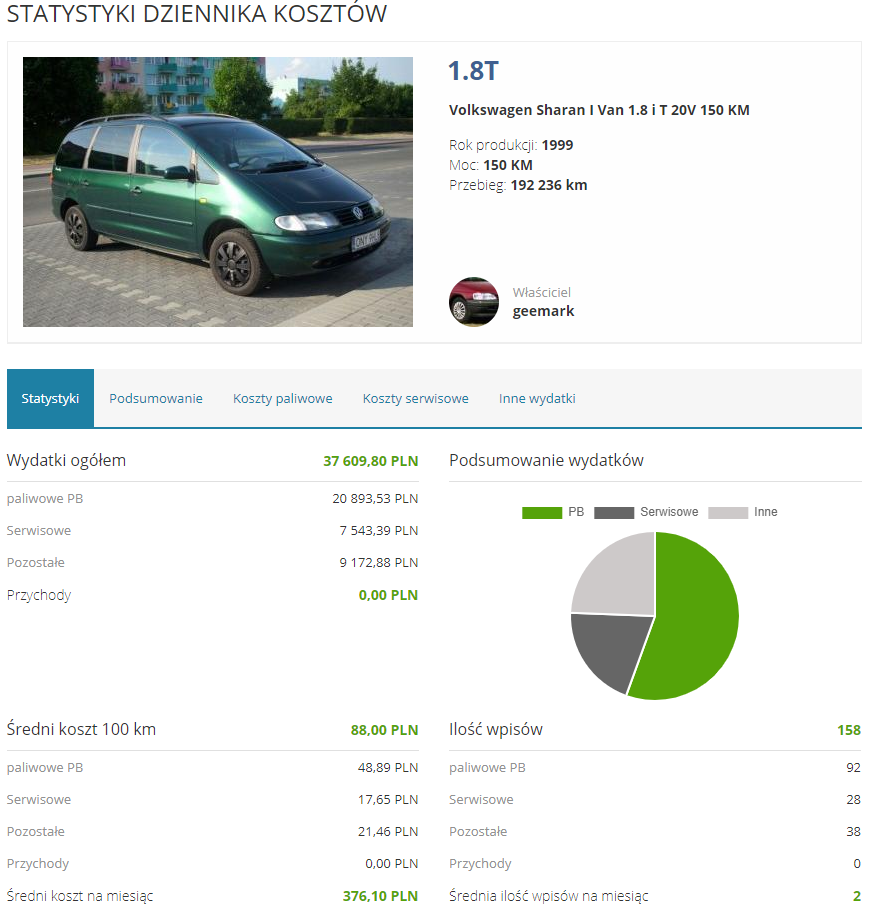
\includegraphics[scale=0.5]{autocentrum.png}
	\caption{Przykładowy wygląd dziennika kosztów ze strony \textit{www.autocentrum.pl} \cite{autocentrum}}
	\label{autocentrum}
\end{figure}
\begin{figure}[H]
	\centering
		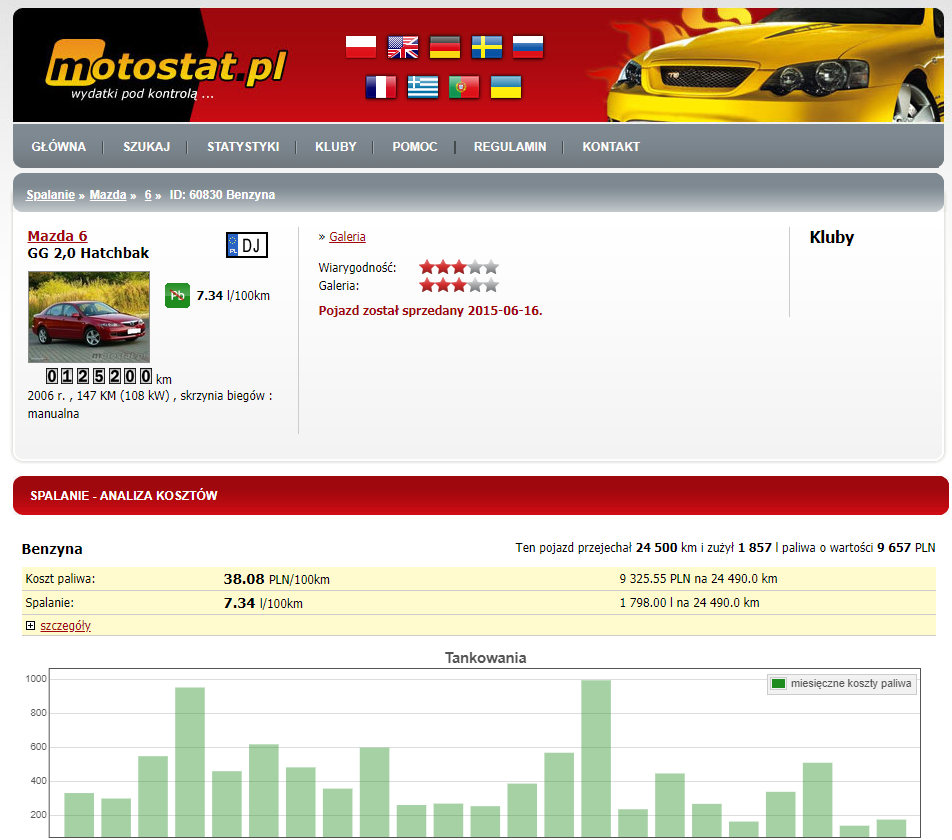
\includegraphics[scale=0.5]{motostat.png}
	\caption{Przykładowy wygląd dziennika kosztów ze strony \textit{www.motostat.pl} \cite{motostat}}
	\label{motostat}
\end{figure}

Żadna z wyżej wymienionych aplikacji w żaden sposób nie weryfikuje wprowadzanych wpisów dotyczących pojazdów. Bieżący projekt ma na celu usprawnienie aplikacji obecnych dotychczasowo na rynku o funkcję weryfikacji wpisów. Każda informacja dodawana do systemu przez użytkownika będzie wymagała obowiązkowo podania obecnego przebiegu. Przebieg ten będzie można dodatkowo potwierdzić zamieszczając zdjęcie licznika pojazdu. Dodatkowo w celu zwiększenia wiarygodności wpisy dodawane przez serwis samochodowy będą wyróżnione, dzięki czemu właściciele pojazdów będą chętniej oddawać pojazdy do naprawy wykwalifikowanym serwisom zamiast własnoręcznie naprawiać samochód. Zwiększą tym samym wiarygodność ich historii pojazdu.

\begin{figure}
	\centering
		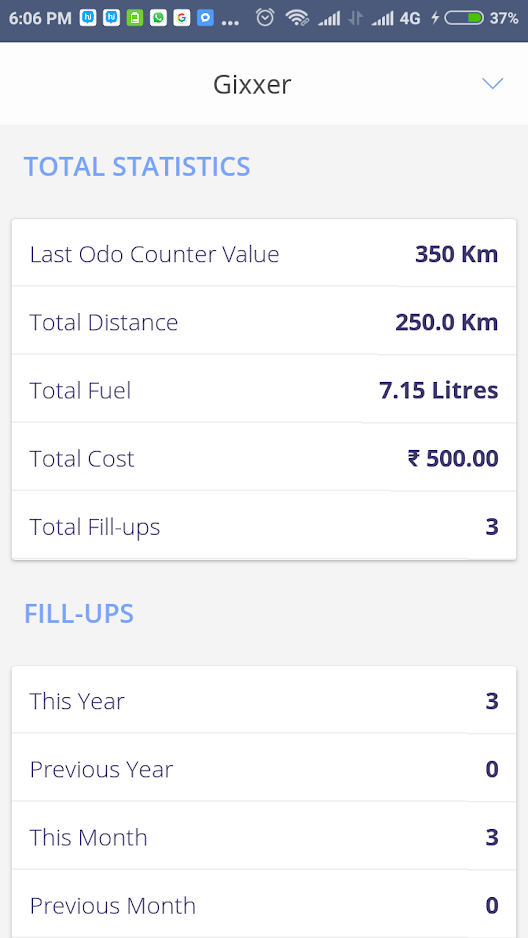
\includegraphics[scale=0.5]{mob1.png}
		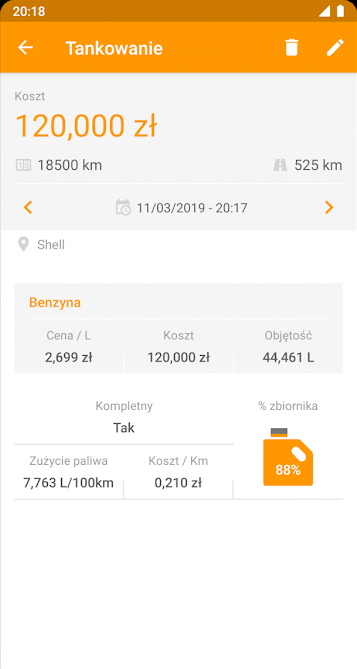
\includegraphics[scale=0.7]{mob2.png}
	\caption{Przykładowy wygląd dziennika kosztów aplikacji \textit{Fuel Buddy} \cite{fuel} oraz \textit{Drivvo} \cite{drivvo}}
	\label{mob}
\end{figure}


 


%---------------------------------------------------------
%					Część czwarta
%---------------------------------------------------------
\newpage
\section{Narzędzia i technologie zastosowane w projekcie}

System wykorzystuje następujące technologie: \textit{Firebase} \cite{firebase}, \textit{Flutter} \cite{flutter}, \textit{React JS} \cite{react} i~\textit{Bootstrap} \cite{bootstrap}. Diagram systemu oraz wykorzystanych technologi został przedstawiony na rysunku \ref{technologie}.

\begin{figure}[H]
	\centering
		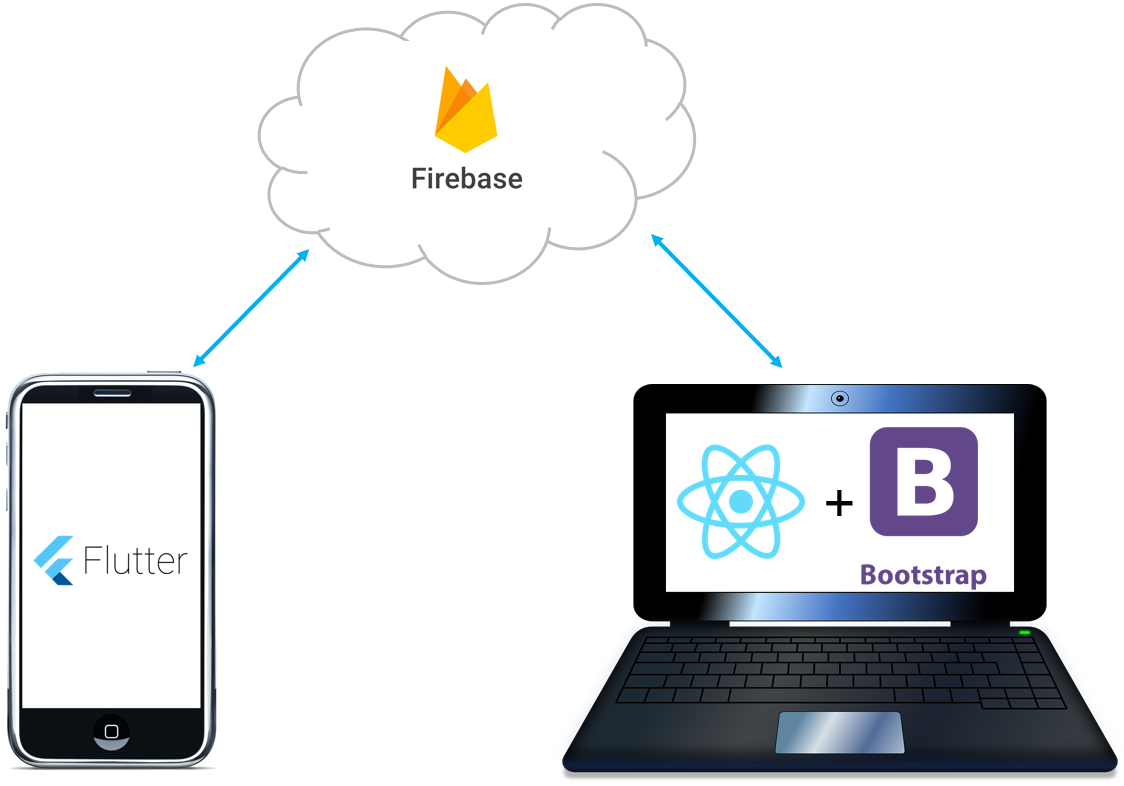
\includegraphics[scale=0.52]{technologie.png}
	\caption{Technologie wykorzystane w systemie}
	\label{technologie}
\end{figure}

Centralnym punktem całego systemu jest baza danych umieszczona w \textit{Firebase}. Jest to darmowe narzędzie od firmy \textit{Google} służące do tworzenia aplikacji mobilnych oraz webowych. Stanowi backend dla aplikacji webowej oraz mobilnej, dzięki czemu tworząc aplikacje należy skupić się tylko na odpowiednim modyfikowaniu i wyświetlaniu zgromadzonych danych.

Do stworzenia aplikacji mobilnej został wykorzystany \textit{Flutter}. Jest to jeszcze świeże rozwiązanie programistyczne opracowane również przez firmę \textit{Google}, które pozwala na jednoczesne tworzenie aplikacji na Androida oraz iOS. Oznacza to, że nie trzeba pisać dwóch oddzielnych aplikacji na dwa wiodące mobilne systemy operacyjne. Jest to spore ułatwienie oraz duża oszczędność czasu.

Za wygląd aplikacji webowej odpowiada \textit{React JS} oraz \textit{Bootstrap}. Obydwa rozwiązania są udostępnione na licencji MIT. Oznacza to że użytkownik ma prawo do używania, kopiowania, modyfikowania i rozpowszechniania (w tym sprzedaży) oryginalnego lub zmodyfikowanego programu w postaci binarnej lub źródłowej. \textit{React JS} w połączeniu z \textit{Bootstrap}'em pozwalają w łatwy sposób tworzyć interfejs graficzny strony oraz aplikacje internetowe. \textit{Bootstrap} pozwala na wygodne stylizowanie elementów strony dzięki czemu aplikacje webowe mogą być responsywne. Oznacza to że strona internetowa automatycznie dostosowuje się do wielkości ekranu na jakim się wyświetla. 




%---------------------------------------------------------
%					Część piąta
%---------------------------------------------------------
\newpage
\section{Kamienie milowe i plan projektu}

\noindent Na rysunku \ref{gantt} został przedstawiony wykres Gantta zawierający takie etapy jak: 
\begin{itemize}
\item projektowanie,
\item realizacja,
\item testowanie,
\item zakończenie.
\end{itemize}

Etap projektowania zawiera wszystkie czynności związane z planowaniem funkcjonalności oraz wyglądu systemu. Na tym etapie zostały zapisane wszystkie wymagania dotyczące funkcjonowania systemu oraz narysowane prototypowe szkice wyglądu aplikacji webowej i~mobilnej. Podczas pierwszego spotkania projektowego funkcjonalności zostały podzielone na podstawowe i rozszerzone. Głównym priorytetem było wykonanie funkcjonalności podstawowych.

Drugim etapem była realizacja. W tej fazie została napisana aplikacja webowa oraz mobilna zgodnie z założeniami zapisanymi w poprzednim etapie realizacji projektu. Na tym etapie zostały również wprowadzone pierwsze poprawki dotyczące planowanego wyglądu oraz funkcjonowania systemu. Był to najdłuższy etap całego projektu.

Następną częścią realizacji projektu będą testy aplikacji webowej oraz mobilnej.  Na tym etapie zostały naprawione wszystkie błędy, które zostały wykryte podczas testowania aplikacji. Oprócz naprawy błędu zostały wprowadzone drobne ulepszenia poprawiające wygląd aplikacji. 

Ostatnią fazą było zakończenie projektu. Na tym etapie został przedstawiony gotowy produkt zawierający działającą aplikację mobilną oraz webową wraz z niezbędną dokumentacją powykonawczą. 

	\begin{figure}[H]
		\centering
		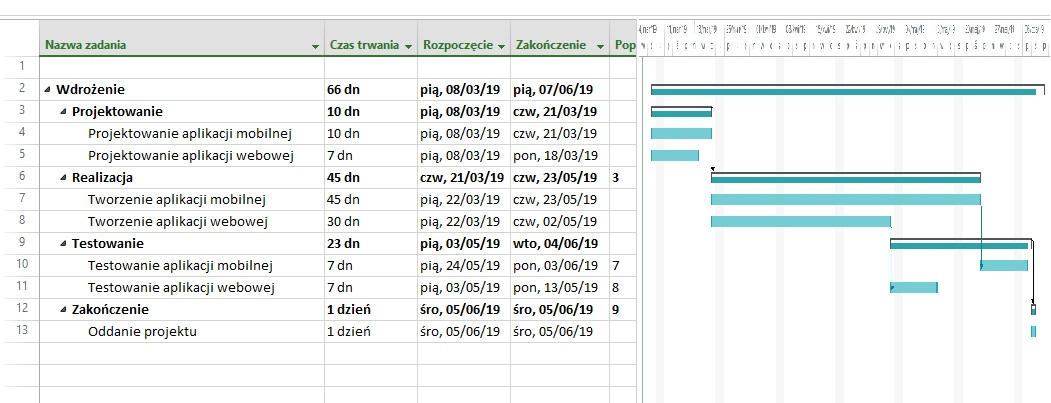
\includegraphics[scale=0.75, angle=270]{wykres_ganttaV3.png}
		\caption{Wykres Gantta}
		\label{gantt}
	\end{figure}
	

Kalkulacja kosztów oraz nakładów pracy potrzebnej do realizacji projektu została przedstawiona w tabeli \ref{kosztorys}. Uwzględnia on koszt rzeczywistego czasu pracy pięciu osób wraz z~kosztem ubezpieczenia i podatkiem VAT.

\begin{table}[H]
\begin{center}
\captionof{table}{Kosztorys}
\label{kosztorys}
	\begin{tabular}{|p{0.55\linewidth}|p{0.15\linewidth}|}%{|l|l|}
	\hline
	Liczba osób 	& 5 				\\ \hline
	Średni czas pracy jednej osoby w godzinach		& 60\\ \hline
	Ilość roboczogodzin & 300	\\ \hline
	Koszt pracy (300h*80zł) & 24000	\\ \hline
	Koszt ubezpieczenia (19.64\%) & 4714	\\ \hline
	Całkowity koszt bezpośredni & \textbf{28714}	\\ \hline
	Koszt pośredni (20\%) & 5743\\ \hline
	Całkowity koszt & 34456\\ \hline
	Zysk & 0\\ \hline
	Podatek VAT (23\%) & 7925\\ \hline
							 \hline
	Koszt produktu & \textbf{42381zł}\\ \hline
	\end{tabular}
\end{center}
\end{table}


%---------------------------------------------------------
%					Część szósta
%---------------------------------------------------------
\newpage
\section{Opis implementacji i wdrożenia projektu}


Baza danych została umieszczona w \textit{Firebase}. W niej przechowywane są informacje o~użytkownikach oraz o ich pojazdach i naprawach. Informacje te w celu zwiększenia bezpieczeństwa zostały zahaszowane algorytmem kryptograficznym md5. Fragment bazy danych został pokazany na rysunku \ref{baza}.

	\begin{figure}[H]
		\centering
		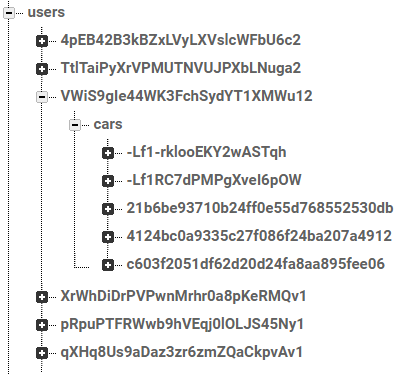
\includegraphics[scale=1]{baza_danych.png}
		\caption{Fragment bazy danych}
		\label{baza}
	\end{figure}

Aplikacja mobilna została napisana przy użyciu narzędzia programistycznego \textit{Flutter}. Dzięki temu powstała jednocześnie aplikacja na system operacyjny \textit{Android} oraz \textit{iOS}. Wygląd aplikacji mobilnej przedstawia rysunek \ref{app_mobilna}. W celu zainstalowania aplikacji na telefon z~systemem \textit{Android} wystarczy umieścić plik \textit{.apk} z aplikacją na telefonie, a następnie poprzez menadżera plików zainstalować aplikację.

	\begin{figure}[H]
		\centering
		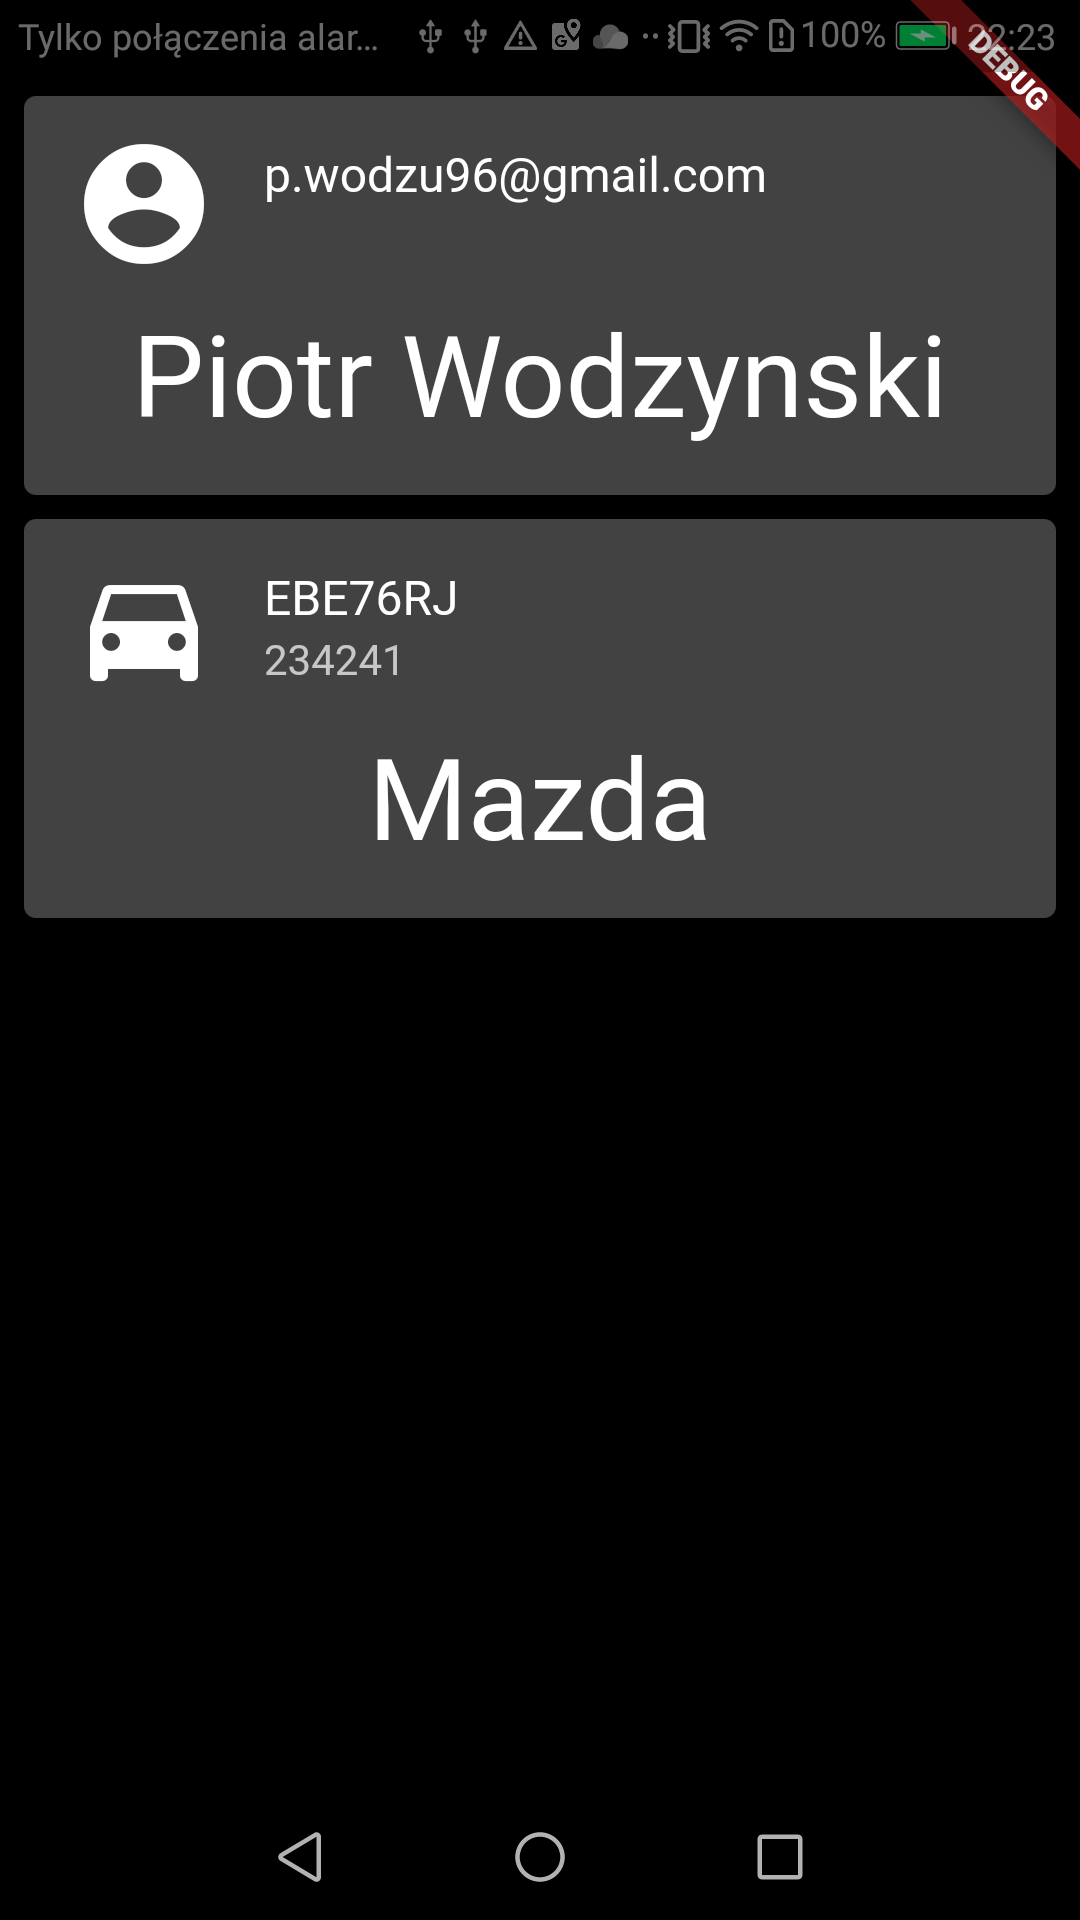
\includegraphics[scale=0.21]{app_mobilna1.png}
		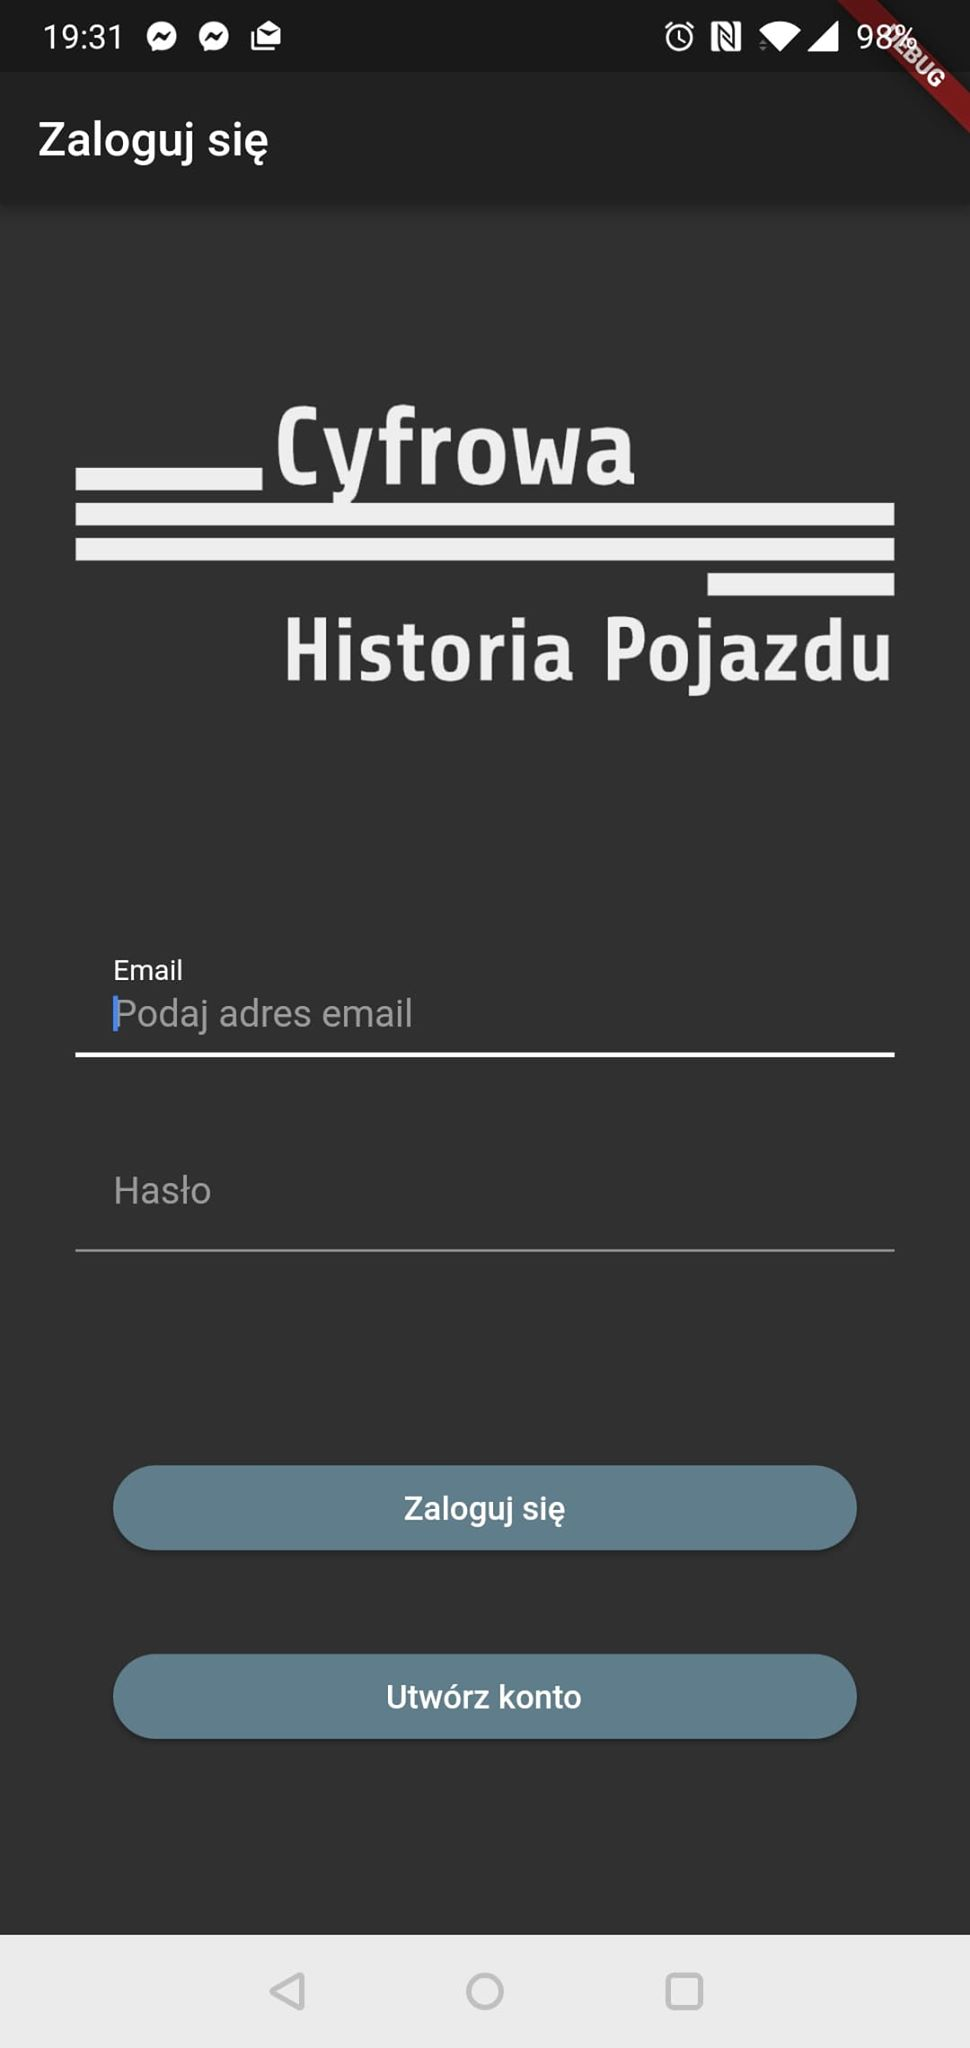
\includegraphics[scale=0.20]{app_mobilna2.png}
		\caption{Wygląd aplikacji mobilnej}
		\label{app_mobilna}
	\end{figure}

Aplikacja webowa została napisana przy użyciu narzędzia \textit{React JS} oraz \textit{Bootstrap}.
Do uruchomienia serwera, na którym będzie znajdowała się nasza strona potrzebne jest narzędzie \textit{Node.js} w wersji 10+. Aby to zrobić należy wejść do głównego folderu aplikacji i w wierszu poleceń wpisać kolejno komendy: \textit{npm install, npm start}. Po poprawnym uruchomieniu nasza aplikacja pojawi się na adresie \textit{localhost:3000}. Wygląd aplikacji webowej przedstawia rysunek  \ref{app_webowa1} i \ref{app_webowa2}.

	\begin{figure}[H]
		\centering
		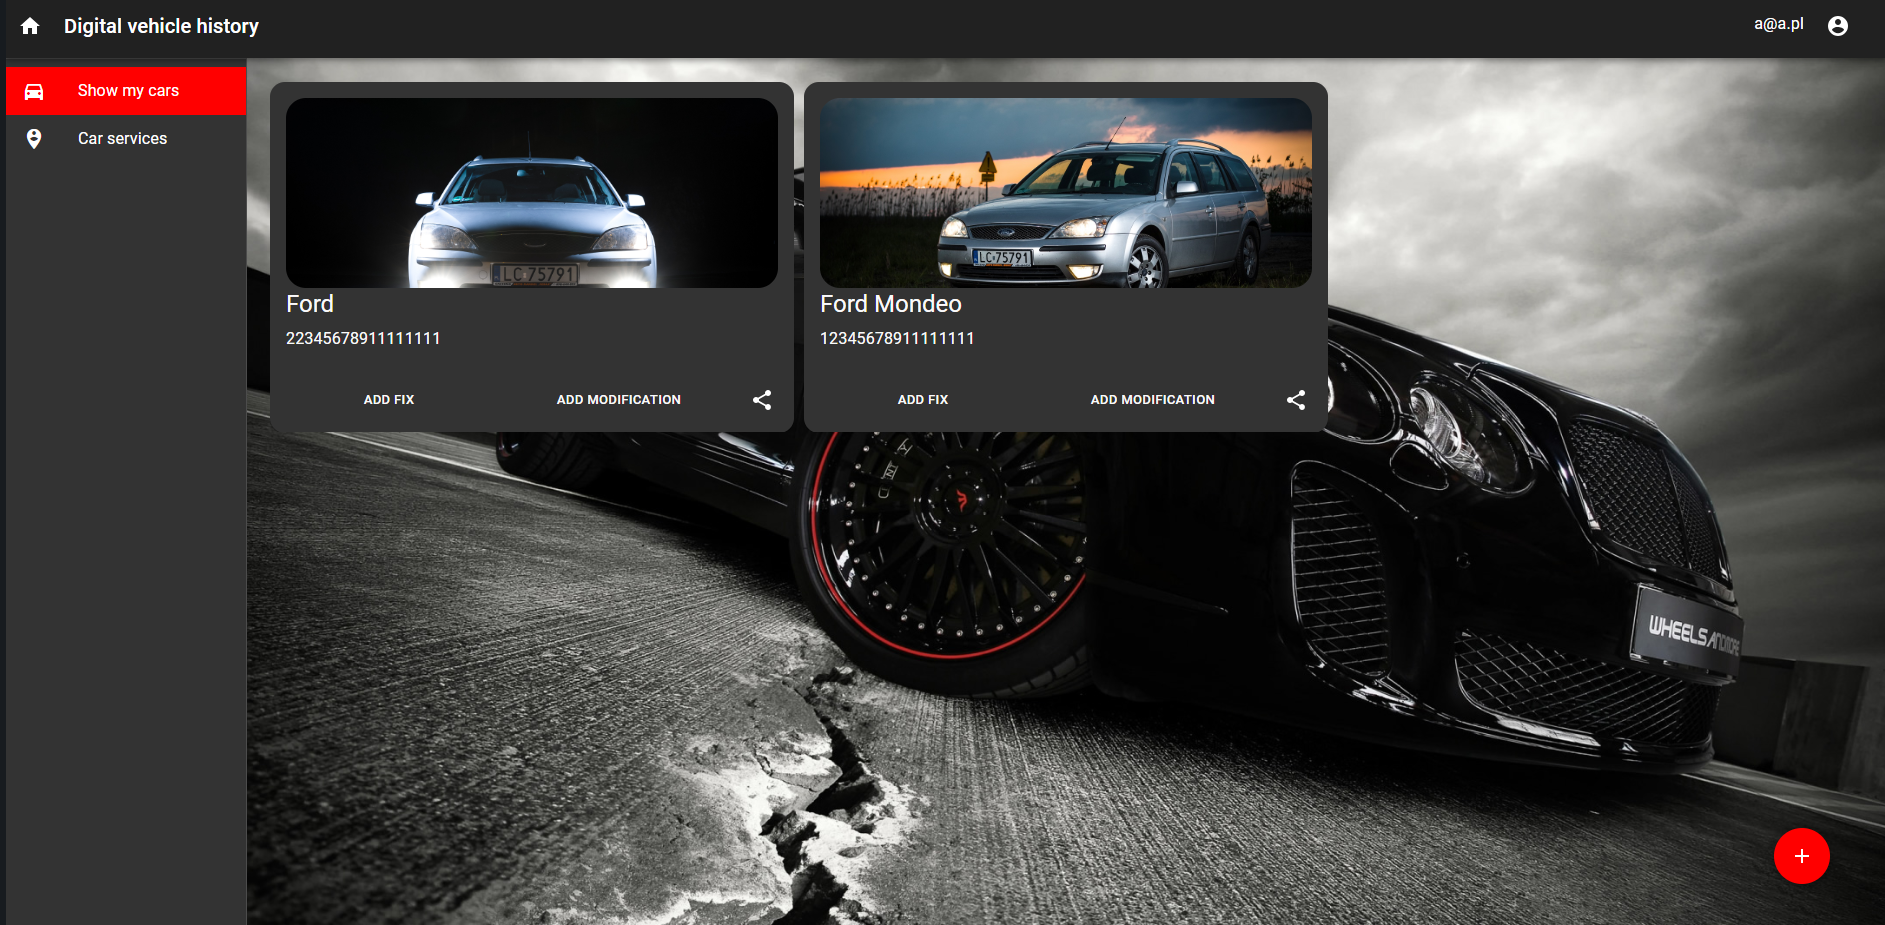
\includegraphics[scale=0.33]{app_web1.png}
		\caption{Wygląd aplikacji webowej}
		\label{app_webowa1}
	\end{figure}
		\begin{figure}[H]
		\centering
		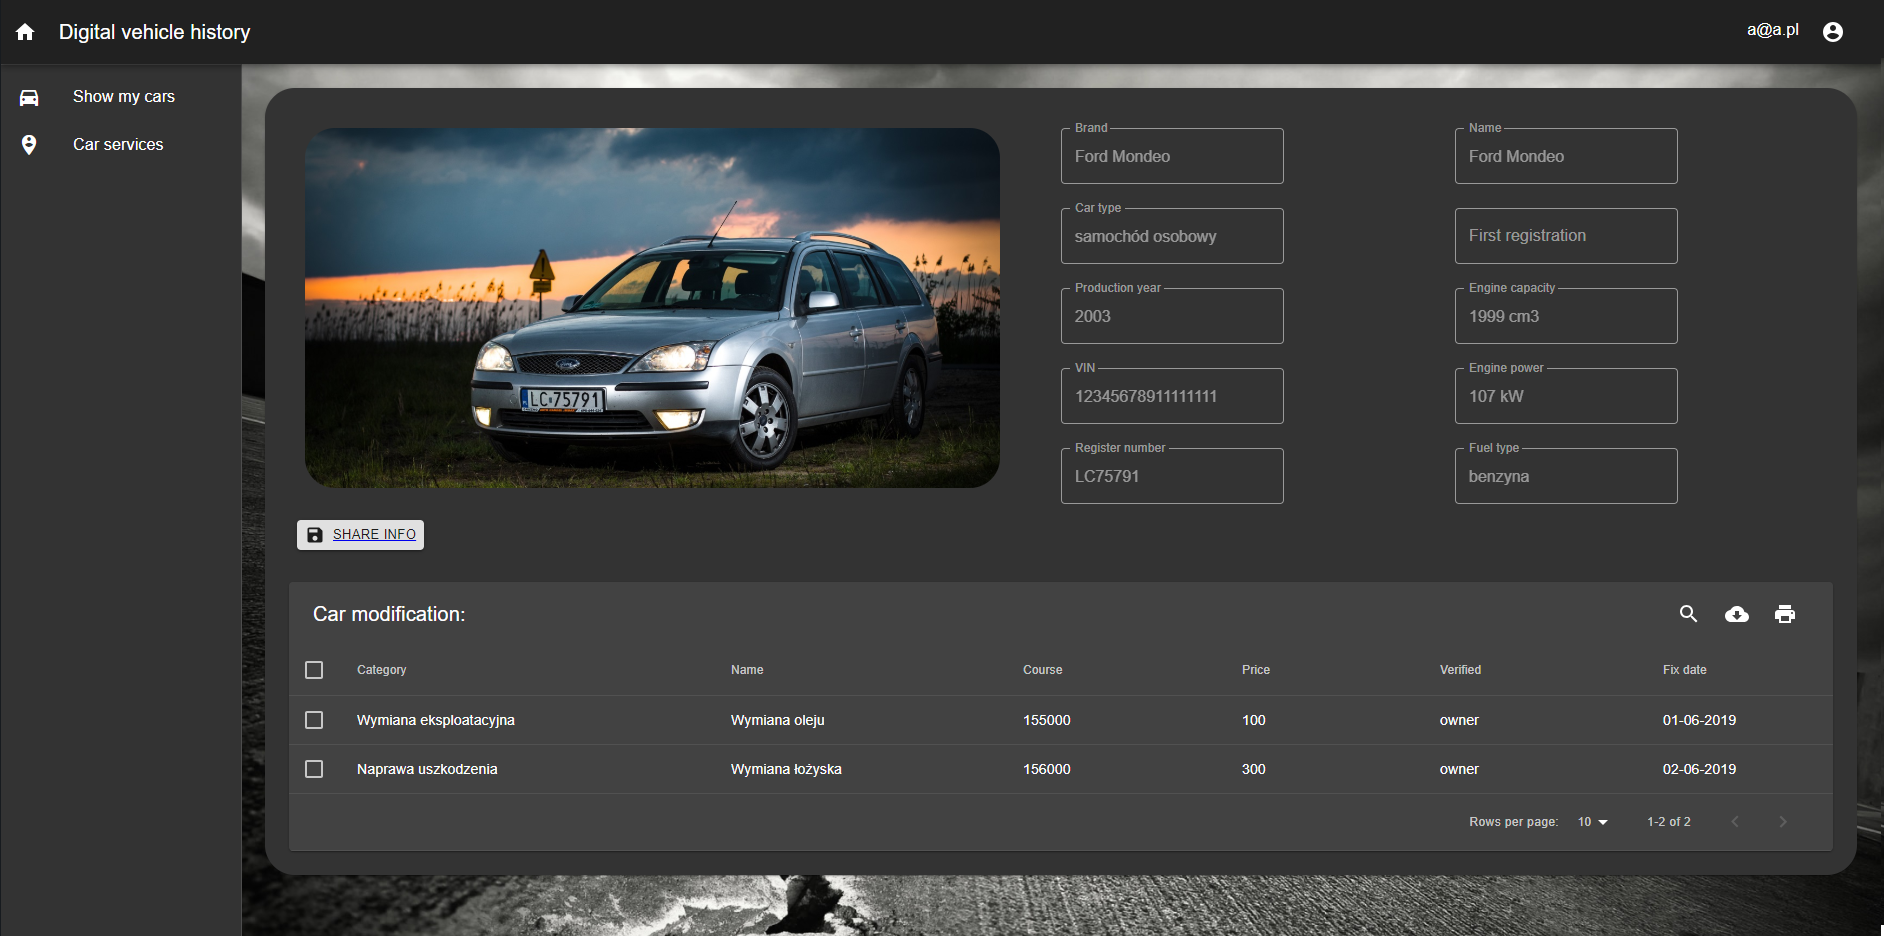
\includegraphics[scale=0.33]{app_web2.png}
		\caption{Wygląd aplikacji webowej}
		\label{app_webowa2}
	\end{figure}

React.js jest to biblioteka języka Java Script, która jest stosowana do tworzenia interfejsów graficznych aplikacji webowych. Główną cechą, która wyróżnia React.js jest tak zwany wirtualny DOM, czyli Document Object Model. React przechowuje DOM aplikacji w pamięci, następnie po zmianie stanu danego komponentu szuka różnic między widokami zachowanymi w pamięci a tymi na ekranie komputera i w razie potrzeby aktualizuje zmiany. Zakłada się, że Interfejs użytkownika składa się z komponentów. Komponenty w React mogą posiadać lub nie posiadać stanu. Stan jest to zdefiniowany obiekt o nazwie state. W czasie zmiany któregoś z atrybutu następuje ponowne renderowanie. Komponenty te zazwyczaj posiadają sekcję render. W tej sekcji zwracany jest kod JSX, który swoją składnią przypomina HTML, jedna różni się od niej. W komponentach tych mogę również być definiowane funkcję. React korzysta z zasady, że dane płyną w dół. Są one przekazywane poprzez propsy do dzieci. Fragment kodu przedstawia rysunek \ref{web1}.
\begin{figure}[H]
		\centering
		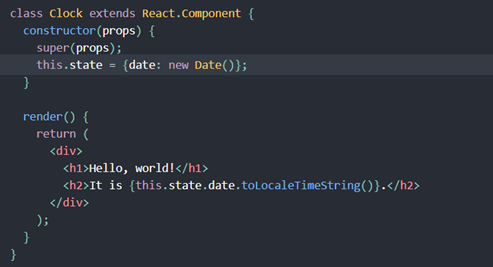
\includegraphics[scale=1]{web1.png}
		\caption{Fragment kodu \textit{React.js}}
		\label{web1}
	\end{figure}
	
Stylowanie komponentów polega na tworzeniu nowych komponentów, przypisując im klasy. Dzięki temu nie ma potrzeby stosowania unikatowych klas CSS-owych w obrębie projektu. Komponent CarCard jest argumentem funkcji styled, która zwraca komponent StyledCarCard z zaaplikowanymi stylami oraz unikalną klasą CSS-ową. Fragment stylizowania przedstawia rysunek \ref{web1}.

 \begin{figure}[H]
		\centering
		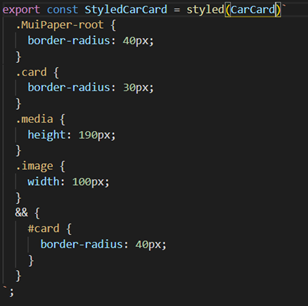
\includegraphics[scale=1]{web2.png}
		\caption{Fragment stylizowania}
		\label{web2}
	\end{figure}
	
W katalogu config definiuje się pliki odpowiedzialne za połączenie do bazy danych (rysunek \ref{web3}). W pliku firebase.js został napisany obiekt konfiguracyjny, który przyjmuję parametry potrzebne do dostępu aplikacji Firebase. Są udostępniane, gdy stworzy się odpowiedni projekt na platformie. 
\begin{itemize}
\item	apiKey
\item	authDoboot
\item	dataBaseURL
\item	projectID
\item	storageBucket
\item	messagingSenderId
\end{itemize}
 \begin{figure}[H]
		\centering
		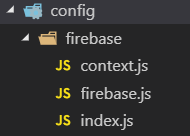
\includegraphics[scale=1]{web3.png}
		\caption{Katalog config}
		\label{web3}
	\end{figure}
	
Plik firebase.js spełnia rolę serwisu http. Udostępnia on metody, odpowiedzialne za zapis do bazy danych, odczyt, edycja, tworzenie użytkowników, logowanie itp. Przykładowa metoda pochodząca z pliku firebase.js, służąca do dodawania nazw serwisów została przedstawiona na rysunku \ref{web4}.

 \begin{figure}[H]
		\centering
		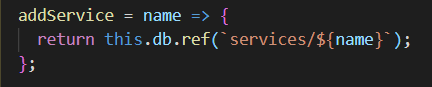
\includegraphics[scale=1]{web4.png}
		\caption{Metoda z pliku firebase.js}
		\label{web4}
	\end{figure}
	
	Plik context.js jest odpowiedzialny za przygotowanie konsumera kontekstu aplikacji (rysunek \ref{web5} i \ref{web6}). Aby korzystać z funkcji dostępnych poprzez skonfigurowanie modułu firebase stworzono kontekst, poprzez osadzenia głównego komponentu aplikacji w tagi Providera. Od teraz każdy komponent, który stanie się konsumerem danego kontekstu będzie miał dostęp do wszystkich metod zdefiniowanych w pliku firebase.js. 
	
	 \begin{figure}[H]
		\centering
		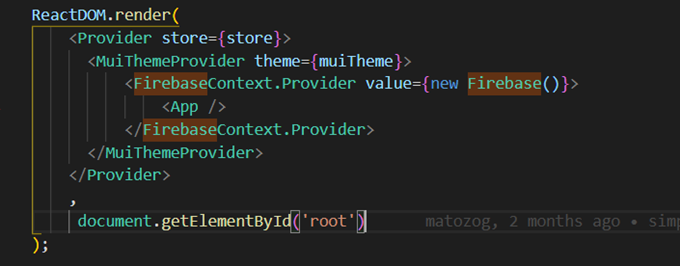
\includegraphics[scale=0.8]{web5.png}
		\caption{Fragment pliku context.js}
		\label{web5}
	\end{figure}
	 \begin{figure}[H]
		\centering
		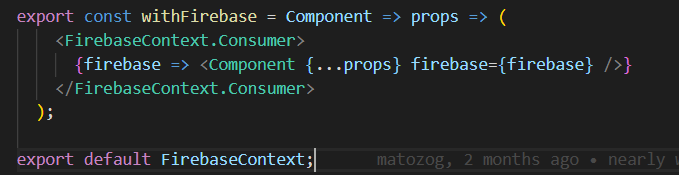
\includegraphics[scale=0.8]{web6.png}
		\caption{Fragment pliku context.js}
		\label{web6}
	\end{figure}

Routing – aplikacja posiada różne strony i podstrony, dlatego konieczne było zaimplementowanie routera (rysunek \ref{web7}). Mechanizm routingu został spełniony przez React Router. Ścieżki zdefiniowane są w pliku jako tablica obiektów, posiadających adresy, ikony, referencje do ścieżek, nazwy oraz rolę dostępu. Jako przykład można pokazać komponent, pokazujący listę samochodów. Dostęp do poszczególnych ścieżek zależny jest od roli użytkownika w~systemie.  
	 \begin{figure}[H]
		\centering
		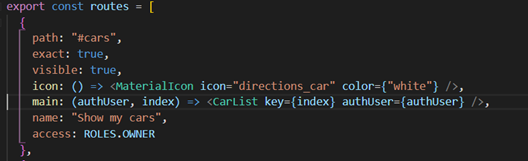
\includegraphics[scale=1]{web7.png}
		\caption{Fragment implementacji routingu}
		\label{web7}
	\end{figure}
	
%---------------------------------------------------------
%					Część siódma
%---------------------------------------------------------
\newpage
\section{Wnioski}

Celem pracy było stworzenie systemu, który będzie umożliwiał w łatwy i wygodny sposób dokumentować historię pojazdów. Projekt został zrealizowany przy użyciu stosunkowo nowych technologi, co pozwoliło poszerzyć naszą wiedzę oraz zdobyć cenne doświadczenia. Wszystkie założenia projektowe zostały spełnione.

Podczas realizacji projektu pojawiały się różne trudności, które były na bieżąco rozwiązywane. Jedną z przeszkód było brak darmowego dostępu do API portalu \textit{historiapojazdu.gov.pl}. Ten problem został rozwiązany poprzez stworzenie własnej testowej bazy pojazdów, w której zostały wpisane ręcznie informacje kilku samochodów. Dzięki temu można było przetestować działanie aplikacji pod kątem autentyczności rejestrowanego pojazdu.

W przyszłości projekt może zostać w łatwy sposób przerobiony tak, aby odczytywał informacje z portalu \textit{historiapojazdu.gov.pl}, dzięki czemu stanie się w pełni funkcjonalny. Projekt przy odpowiedniej promocji mógłby zostać wdrożony w życie i skomercjalizowany tak, aby przynosił korzyści jego twórcom. Dotychczasowe aplikacje, które są dostępne na rynku nie oferują funkcji potwierdzania autentyczności przebiegu pojazdu. System \textit{Cyfrowej historii pojazdu} oferuje podobne funkcjonalności co rozwiązania konkurencji, jednakże jest rozszerzony o możliwość weryfikacji przebiegu pojazdu. Dzięki temu właściciel pojazdu może poświadczyć autentyczność przebiegu swojego pojazdu, a co za tym idzie zwiększyć jego wartość.


\newpage
\renewcommand\refname{Bibliografia}
\addcontentsline{toc}{section}{Bibliografia} %utworzenie w spisie treści pozycji Bibliografia
\begin{thebibliography}{9}

\bibitem{autocentrum}  https://www.autocentrum.pl, [Dostęp: 10.05.2019]

\bibitem{motostat}  https://www.motostat.pl, [Dostęp: 10.05.2019]

\bibitem{fuel} https://mobifolio.net/, [Dostęp: 10.05.2019]

\bibitem{drivvo}  http://www.drivvo.com, [Dostęp: 10.05.2019]

\bibitem{firebase}  https://firebase.google.com, [Dostęp: 2.06.2019]

\bibitem{flutter}  https://flutter.dev, [Dostęp: 2.06.2019]

\bibitem{react}  https://reactjs.org, [Dostęp: 2.06.2019]

\bibitem{bootstrap}  https://getbootstrap.com, [Dostęp: 2.06.2019]
\end{thebibliography}
\end{document}


